\section{Products \label{sect:products}}

The products of DM are not the data products defined in \citeds{LSE-163}, rather they are the artifacts, systems and services  we need to produce those products. \secref{sect:dmarc} outlines the highest level of this for DM while  \appref{sect:prodlist}  defines the complete product tree for DM and it is pictorially represented at a trimmed level in  \figref{fig:prods}.
\citeds{LDM-148} provides a trace of products to requirements, while \appref{sect:prodlist} proves a full list with technical manager, WBS element and product owner for each.
Our primary guiding requirements come from \citeds{LSE-30}, the Observatory System Specification (OSS), with \appref{sect:tracefor} tracing DM requirements \citedsp{LSE-61} to OSS, and \appref{sect:traceback} tracing the relevant OSS requirements to DM.

\begin{figure}[htbp]
	\begin{center}
		 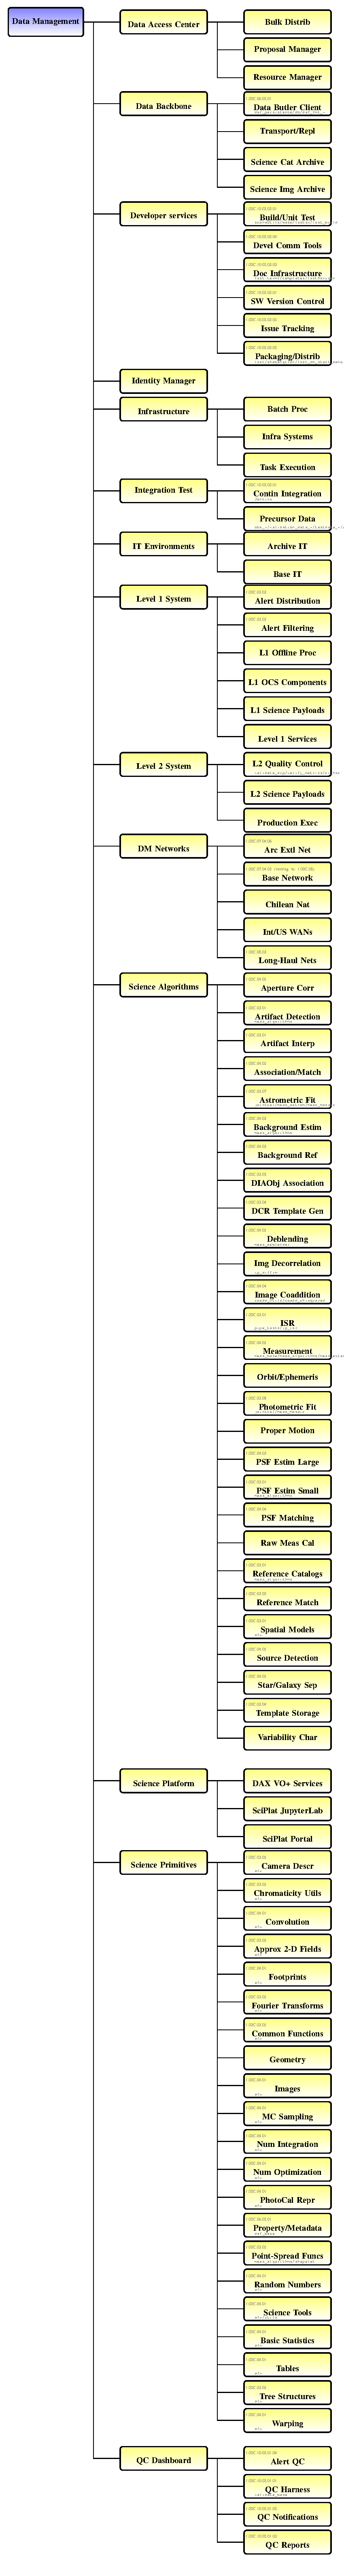
\includegraphics[height=19cm]{ProductTree}
		 \caption{DM product tree. \label{fig:prods}
		 The full list is given in \appref{sect:prodlist}
	 }

	 \end{center}
 \end{figure}

\figref{fig:prods}
 contains the WBS element associated with the component as well as any git repositories belonging to them.
 Since the figure stops at level 3 most git repositories will only be found in the full list in \appref{sect:prodlist}.

 Every git repository should appear in \appref{sect:prodlist}  and hence have a technical manager and product owner identified. The table is hierarchical hence if the manager/owner is not filled in (or the individual is no longer with the project) we may go to the parent element manager/owner. Some work remains to finish rationalizing the components and repositories.

 Every JIRA component should map to one row in \appref{sect:prodlist} thus providing a contact for that component.
 Some JIRA components are not physical products - they should still appear in the \appref{sect:prodlist} which is the single source for DM of component  ownership. Some work is also needed to rationalize the JIRA components.
